\chapter{Introdução}
	Neste capítulo, será feita uma revisão do contexto em que os serviços de bancos de dados em nuvem(em particular, nesse relatório, o serviço Amazon SimpleDB) se apresentam e suas características gerais.
	
\section{Bancos de dados relacionais}
\subsection{História}
	Os bancos de dados relacionais foram introduzidos na década de 1970 em \cite{codd1970} como uma alternativa aos modelos \textit{de navegação}\cite{wikiNavDb}. Os sistemas de bancos de dados que seguiam os modelos de navegação(presentes na década de 1960) apresentavam ao programa cliente a capacidade de percorrer um conjunto de dados segundo um esquema de lista encadeada, onde os dados requisitados pelo programa eram encontrados seguindo-se uma cadeia de referências e verificando se o objeto atualmente referenciado possui a propriedade buscada --- não apresentando, portanto, funcionalidade de busca(a própria aplicação é responsável por filtrar os dados desejados).\\\\
	O conceito apresentado por Codd foi implementado pela IBM em seu SGBD \textit{System R}, que também foi o primeiro a apresentar, em 1978, o uso da então padronizada linguagem de consulta \textbf{SQL}. Constatada a viabilidade e superioridade dos sistemas de bancos de dados relacionais em relação às demandas existentes, várias outras empresas passaram a implementar seus SGBDs comerciais baseando-se no modelo relacional. Entre as principais, figuram \textbf{Oracle}(com o SGBD homônimo), Microsoft(com o \textbf{Microsoft SQL Server}) e ainda a IBM(com seu \textbf{DB2}, derivado do System R). \\\\
	Alternativamente, surgiram também implementações disponíveis para uso gratuito: na Suécia, foi iniciado o projeto \textit{open source} \textbf{MYSQL} por Michael Widenius \cite{wikiMySQL}; na Universidade de Berkeley, em um projeto liderado por Michael Stonebraker, criou-se o SGBD \textbf{PostgreSQL}(o nome vem do fato dele ter se baseado no antigo projeto \textbf{Ingres}, ou seja, \textit{Post Ingres} \cite{wikiPSql})
\\\\\\\\\\

\subsection{Características}
	No sistema proposto por Codd, os dados se organizavam em \textit{tabelas} com entradas de tamanho fixo, não em uma lista de referências como proposto no modelo de navegação. Cada entrada em uma tabela conteria atributos e um certo subconjunto(possivelmente próprio) desses atributos identificaria unicamente uma entrada nessa tabela.\\\\
	Um dos problemas que o modelo de Codd se propunha a resolver era a representação de dados \textit{esparsos}: isto é, como representar e armazenar de maneira eficiente dados que possam apresentar entradas ou atributos vazios. No modelo de navegação, a solução para esse cenário é o uso de um marcador específico para denotar que o atributo está vazio, o que é bastante ineficiente em termos de armazenamento. O modelo relacional, por sua vez, sugeria colocar esses atributos que tinham a possibilidade de serem vazios em uma tabela separada daquela em que se encontra a entrada à qual eles se referem. \\\\
	Por exemplo, suponha que nossos dados consistam de um cadastro onde as pessoas podem ou não fornecer um telefone para contato. Esses dados seriam representados como uma duas tabelas: uma contendo uma entrada para cada pessoa com as respectivas informações pessoas e a outra contento, em cada entrada, um número de telefone e uma \textit{referência} para a entrada na primeira tabela cuja pessoa forneceu aquele número(ver figura \ref{fig:tabelarelacao}).
\begin{figure}[h]
    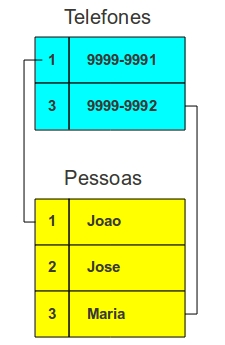
\includegraphics[scale=0.50]{figuras/relacional1.jpg}
    \caption{Tabelas inter-relacionadas}
    \label{fig:tabelarelacao}
\end{figure}
	\\
	Uma característica que se tornou peculiar nos SGBDs relacionais, apesar de não fazer parte da proposta original do modelo relacional, foi o uso de uma linguagem de consulta interpretada pelo SGBD para a extração de dados, a \textbf{SQL}(\textit{Structured Query Language}). Baseada na álgebra relacional, ela permite realizar operações de busca e atualização sobre as tabelas e os dados contidos no banco expressando-se de maneira declarativa sobre \textbf{conjuntos} de dados. Dessa forma, o programa cliente não recupera dados do SGBD através de chamadas a uma \textit{API}, mas sim submetendo consultas SQL que serão interpretadas pelo SGBD.
\\\\\\\\